%%
%%
%%   LaTeX Beamer for ESS Presentation template
%%
%%   Jeong Han Lee, han.lee@esss.se
%%
%%   v0.1 created Monday, Monday, November 23 09:07:19 CET 2015, jhlee
%%
%%

\documentclass[
  9pt
  , table
  , ignorenonframetext
]{beamer}


\usepackage{esstex} 

\meetingname{ESS WS ACQ SYS PDR}
\meetingcity{Trieste}
\meetingcountry{Italy}
\totalpagenumber{\inserttotalframenumber}
%\totalpagenumber{13+}



\title{ESS ICS Presentation; focus on the WS development}
\author{Jeong \textbf{Han} Lee on behalf of ESS ICS}%\inst{1}}
\institute{
  Integrated Control System Division\\
  \textbf{ESS}, Sweden
}
\date{June 28, 2016}


\begin{document}
 
\begin{frame}[plain]
  \titlepage
\end{frame}


\begin{frame}{The Integrated Control System (ICS)}
  \begin{block}{ICS Scope}
    \begin{itemize}
    \item Conventional facilities control integration : power distribution, cooling water, etc
    \item The accelerator control system
    \item The Neutron target control system
    \item EPICS layer for the neutron instruments (in cooperation with the colleagues from science directorate)
    \item Global systems : control network and servers, timing and event systems, and protection \& safety systems
    \end{itemize}
  \end{block}
  \begin{exampleblock}{Combination of}
    \begin{itemize}
    \item On-site developments 
    \item In-kind contributions (up to 50\% of total value)
    \end{itemize}
  \end{exampleblock}
\end{frame}



\begin{frame}{EPICS Environment}
  There is no generic EPICS environment, and each lab has its own environment historically. Historically, many labs use more than one EPICS release and drivers should be built for all EPICS releases in parallel
  \begin{block}{Loadable Driver Module (LDM) at PSI}
    \begin{itemize}
    \item Build drivers for multiple releases of EPICS, and load drivers dynamically from startup script.
    \item is used to run PSI machine since 2005, which is the first presentation in the community.
    \end{itemize}
  \end{block}

  \begin{exampleblock}{ESS EPICS Environment}
    \begin{itemize}
    \item has been evolved from LDM in cooperation with Dirk Zimoch at PSI.
    \item provides a collection of scripts to develop, build, and deploy an EPICS IOC.
    \item provides customized solutions to run different configurations at the same time and in the same machine, to test next releases of IOCs independently, and to switch the old and new versions of an IOC easily and quickly.
    \end{itemize}
  \end{exampleblock}
\end{frame}

\begin{frame}{Hardware Strategy}
  \begin{block}{Generic IOs}
    \begin{itemize}
    \item Fast real-time processing, FPGAs (MTCA.4) : use when strong demands for real-time IO (high cost), FMC and RTM cards
    \item Real-time industrial-type I/O : EtherCAT on IOC (Low cost, distributed, moderate speed -e.g. up to 100 kSPS A/D conversion)
    \item Process I/O with no tight syncronzation requirements : Siemens PLCs (Safety)
    \end{itemize}
  \end{block}
 \begin{exampleblock}{Specific IOs}
    \begin{itemize}
    \item Timing / Event System : Micro-Research Finland 
    \item Motion Control :  DeltaTau Geobrick and EtherCAT Open source SW Bus mater with Beckhoff HW
    \item Serial \& Network-based devices : Ethernet or RS-242/485 serial ports 
    \end{itemize}
  \end{exampleblock}
  
\end{frame}


\begin{frame}{Digital Front-End Platform}
  \begin{itemize}
  \item MTCA.4 AMC with a FPGA, CPU and modular interfaces
  \item In-kind contribution from Switzerland; PSI and the company IOxOS SA
  \item Based on an existing architecture (IFC 1210)
    \begin{itemize}
    \item FPGA and a CPU connected with PCI Express
    \item FMC carrier (FMC: I/O card directly connected to a FPGA)
    \item Deployed, base board for the SwissFEL @ PSI
    \item Refresh components (newer models) and change form factor to MTCA.4
    \end{itemize}
  \end{itemize}
  \begin{exampleblock}{Starter Kit for WS ACQ}
    \begin{itemize}
    \item ELMA VME crate, Type 39 Horizontal, 4 U, 84 HP 
    \item IOXOS IFC1210-A0 with 2 FMC slots
    \item MRF VME-EVG-230 / MRF VME-EVR-230RF
    \item D-tAcq ACQ420FMC-4-\textbf{2000}-16 / D-tAQ ACQ420 TERM01 board / D-tAcq BNC to PTB flying lead
     \end{itemize}
  \end{exampleblock}
\end{frame}



\begin{frame}{Motion Control - MPS integation}
  \begin{columns}
    \begin{column}{.6\textwidth}
      \begin{block}{MCU 1013 - Single Axis MPS version}
        \begin{itemize}
        \item CPU, couplier, linear stage, INC encoder, redundant switches
        \item Motion control with an Open Source EtherCAT master, which is being developed by ICS and the motion group at ESS
        \item Based on the open source EtherCAT technology
        \item The Open Source EtherCAT master (www.etherlab.org) can run on Linux
        \item  No software licences
          %%   \begin{itemize}
          %%   \item EtherCAT hardware have rather high performance
          %%   \item The Open Source EtherCAT master (www.etherlab.org) can run on Linux
          %%   \item No software licences
          %%   \item MCAG group also evaluates an industrial control system called TwinCAT (soft controller running under Windows operating system only) with EtherCAT hardware and the same hardware can be used with this open source approach
          %%   \item ICS is also using open source ethercat master (www.etherlab.org) for sampling analog and digital signals to EPICS. 
          %%   \end{itemize}
        \end{itemize}
      \end{block}
    \end{column}
    \begin{column}{.5\textwidth}
      \centering
      \includegraphics[width=1\textwidth]{./pictures/motion-ws-dual-axis.eps}
      
    \end{column}
    \end{columns}
\end{frame}


%% \begin{frame}{Interface Description \textbf{iff} FW in FE, BE, or Both}
%%   \begin{exampleblock}{Example : Communication}

%%   The Supplier shall provide the required interface to control the XXX remotely. The remote communication protocol shall be compliance with the ESS ICS Standard and the remote communication could be performed through Ethernet networks. The Ethernet interface provides the ability to use TCP socket connection and to fulfill the standard Ethernet attached devices requirements as follows:
  
%% \begin{itemize}
%% \item Ethernet-attached devices shall be compatible with a 1 Gb/s network
%% \item Ethernet-attached devices shall operate at a minimum network speed of 100 Mb/s
%% \item Ethernet-attached devices shall obtain their network address either through static address configuration or DHCP.
%% \item Ethernet-attached devices shall include a Standard RJ-45 modular connector
%% \item Cables should be wired by the Industry Standard Pin-out
%% \end{itemize}
%% \end{exampleblock}
%% \end{frame}


\begin{frame}{Interface Description \textbf{iff} FW in FE, BE, or Both}
  \begin{exampleblock}{Example : Status and Queues}
  A series of status and queues of the unit or any of its components shall be introduced in order to allow the operator to monitor and manipulate the various events. In addition, a series of generic status shall be defined. For example, the following information shall be defined:
  \begin{itemize}
  \item Model (and company) name
  \item HW Serial Number
  \item  Operation Status
  \item  Remote or Local Status
  \item  Front Panel Lock
  \item  Heartbeat
  \item  Error Status
  \item  Firmware Version
  \item  Firmware Update date
  \item  Communication related Settings
  \end{itemize}
\end{exampleblock}
\end{frame}



\begin{frame}{Questions}
  In mathematics the art of proposing a question must be held of higher value than solving it.\\
  \begin{flushright}
    Georg Cantor
  \end{flushright}

  It is not enough for me to ask the question; I want to know how to answer the one question that seems to encompass everything I face: What am I here for?
   \begin{flushright}
    Abraham Joshua-Heschel
   \end{flushright}

   Computers are useless. They can only give you answers.
   \begin{flushright}
     Pablo Picasso 
   \end{flushright}

\end{frame}



%% \begin{frame}{ICS Control System Fact}
%%   \begin{exampleblock}{until 2016.06}
%%     \begin{itemize}
%%     \item 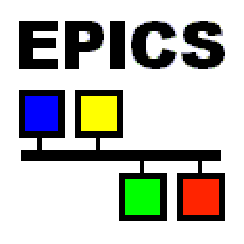
\includegraphics[width=0.06\textheight]{./pictures/epics_logo.eps}~ \textbf{EPICS}, and ESS EPICS Environment
%%     \item 
\includegraphics[width=0.05\textheight]{./pictures/centos-emboss.eps} ~ CentOS 64bit for OS (7.1  1503)
%%     \item 
\includegraphics[width=0.08\textheight]{./pictures/git_logo.eps}~ for sources version control 
%%     \item Event System : MRF EVG/EVR boards (cPCI, PCIe, VME, MTCA, etc)
%%     \item Siemens S7 PLC
%%     \item Control System Studio for OPI
%%     \end{itemize}
%%   \end{exampleblock}
%%   \end{frame}




%% \begin{frame}
%%   \frametitle{A Page for a picture}
%%   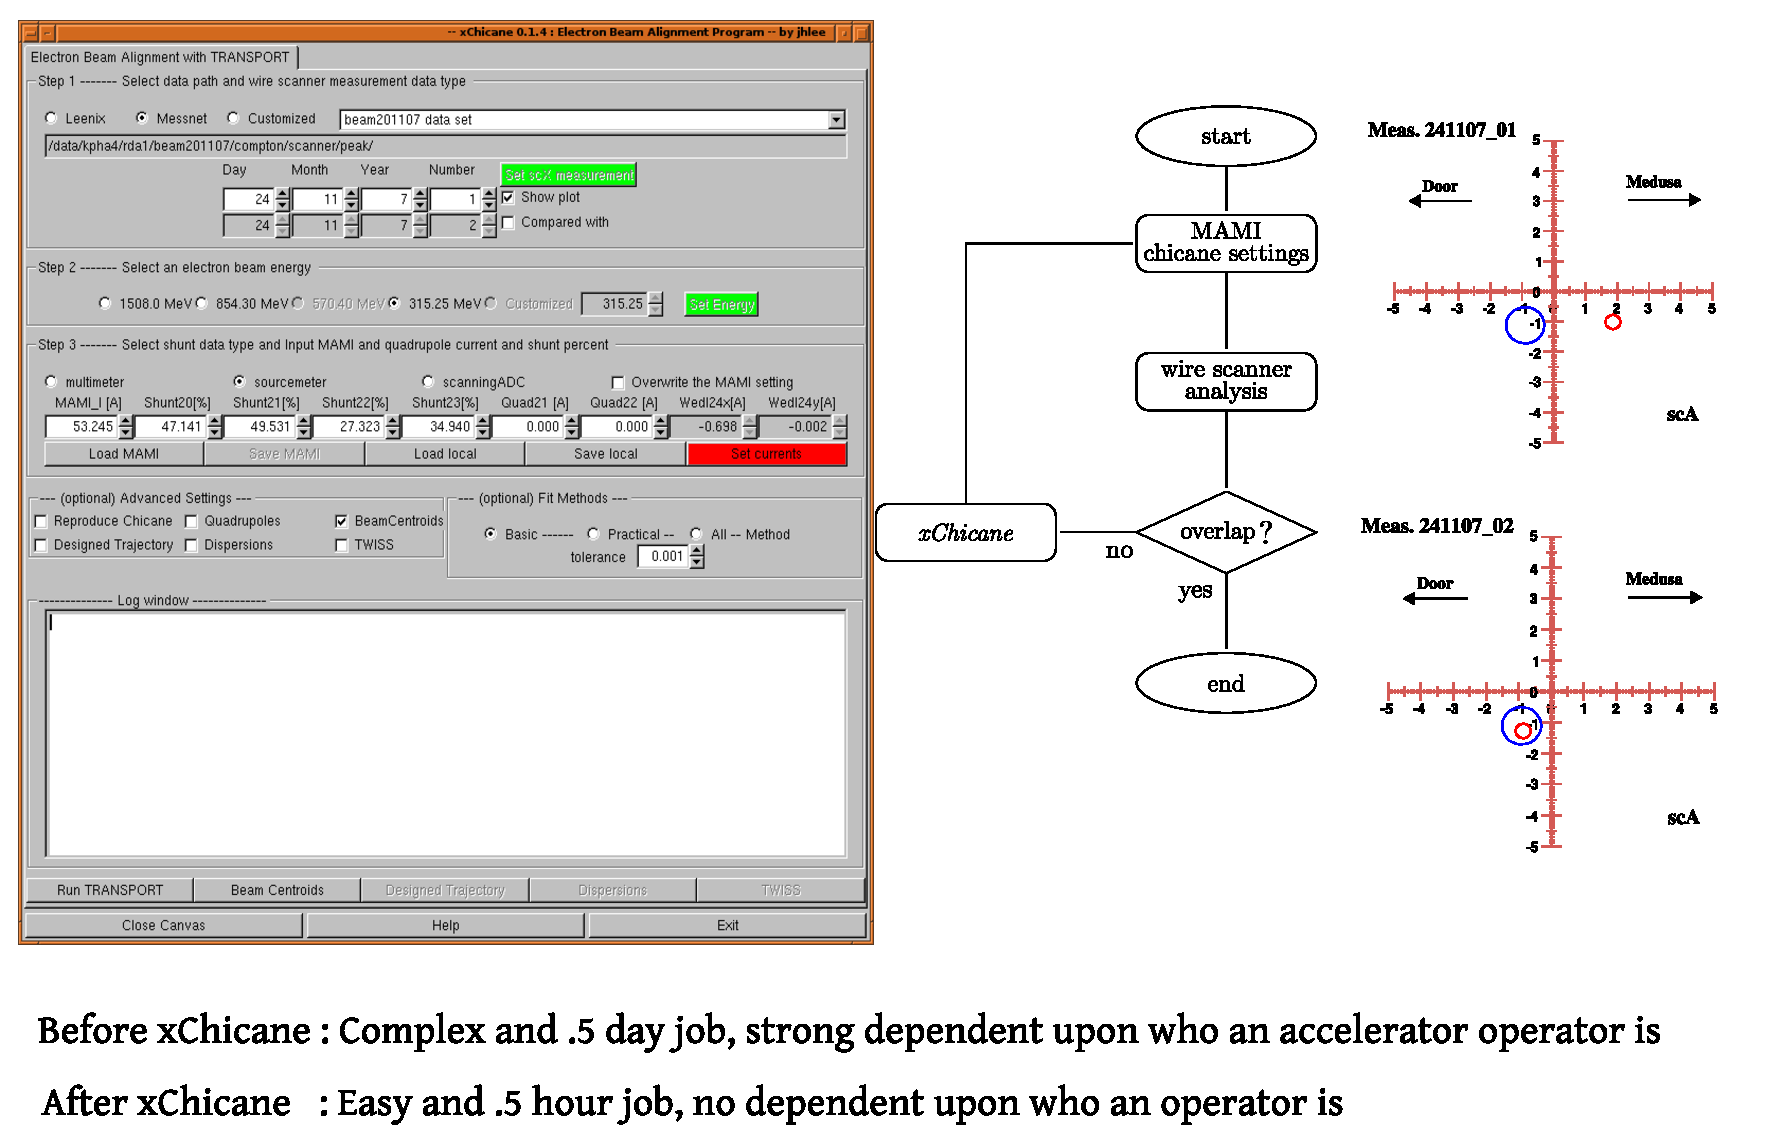
\includegraphics[width=\columnwidth]{./pictures/xchicane.eps}
%% \end{frame}


\begin{frame}[plain]
  \begin{center}
    {\LARGE Grazie!}  \\\vspace{6mm}
    {\LARGE Tack!}  \\\vspace{6mm}
    {\LARGE 감사합니다!}\\\vspace{6mm}
    {\LARGE Thank you!}  \\\vspace{6mm}
    {\LARGE Dankesch\"on!} \\\vspace{6mm}
    {\LARGE ¡Gracias!}\\\vspace{6mm}
%            {\LARGE Merci!}\\\vspace{6mm}
    {\LARGE \smiley } 
  \end{center}
  
\end{frame}


\end{document}
